\documentclass[tikz, margin=10pt]{standalone}

\usepackage{siunitx}
\usepackage[american]{circuitikz}
\usepackage{amsmath}%To allow \cfrac macro
\usepackage{bm}%Bold math
\usetikzlibrary{arrows.meta,decorations.markings,decorations.pathreplacing}

\begin{document}
    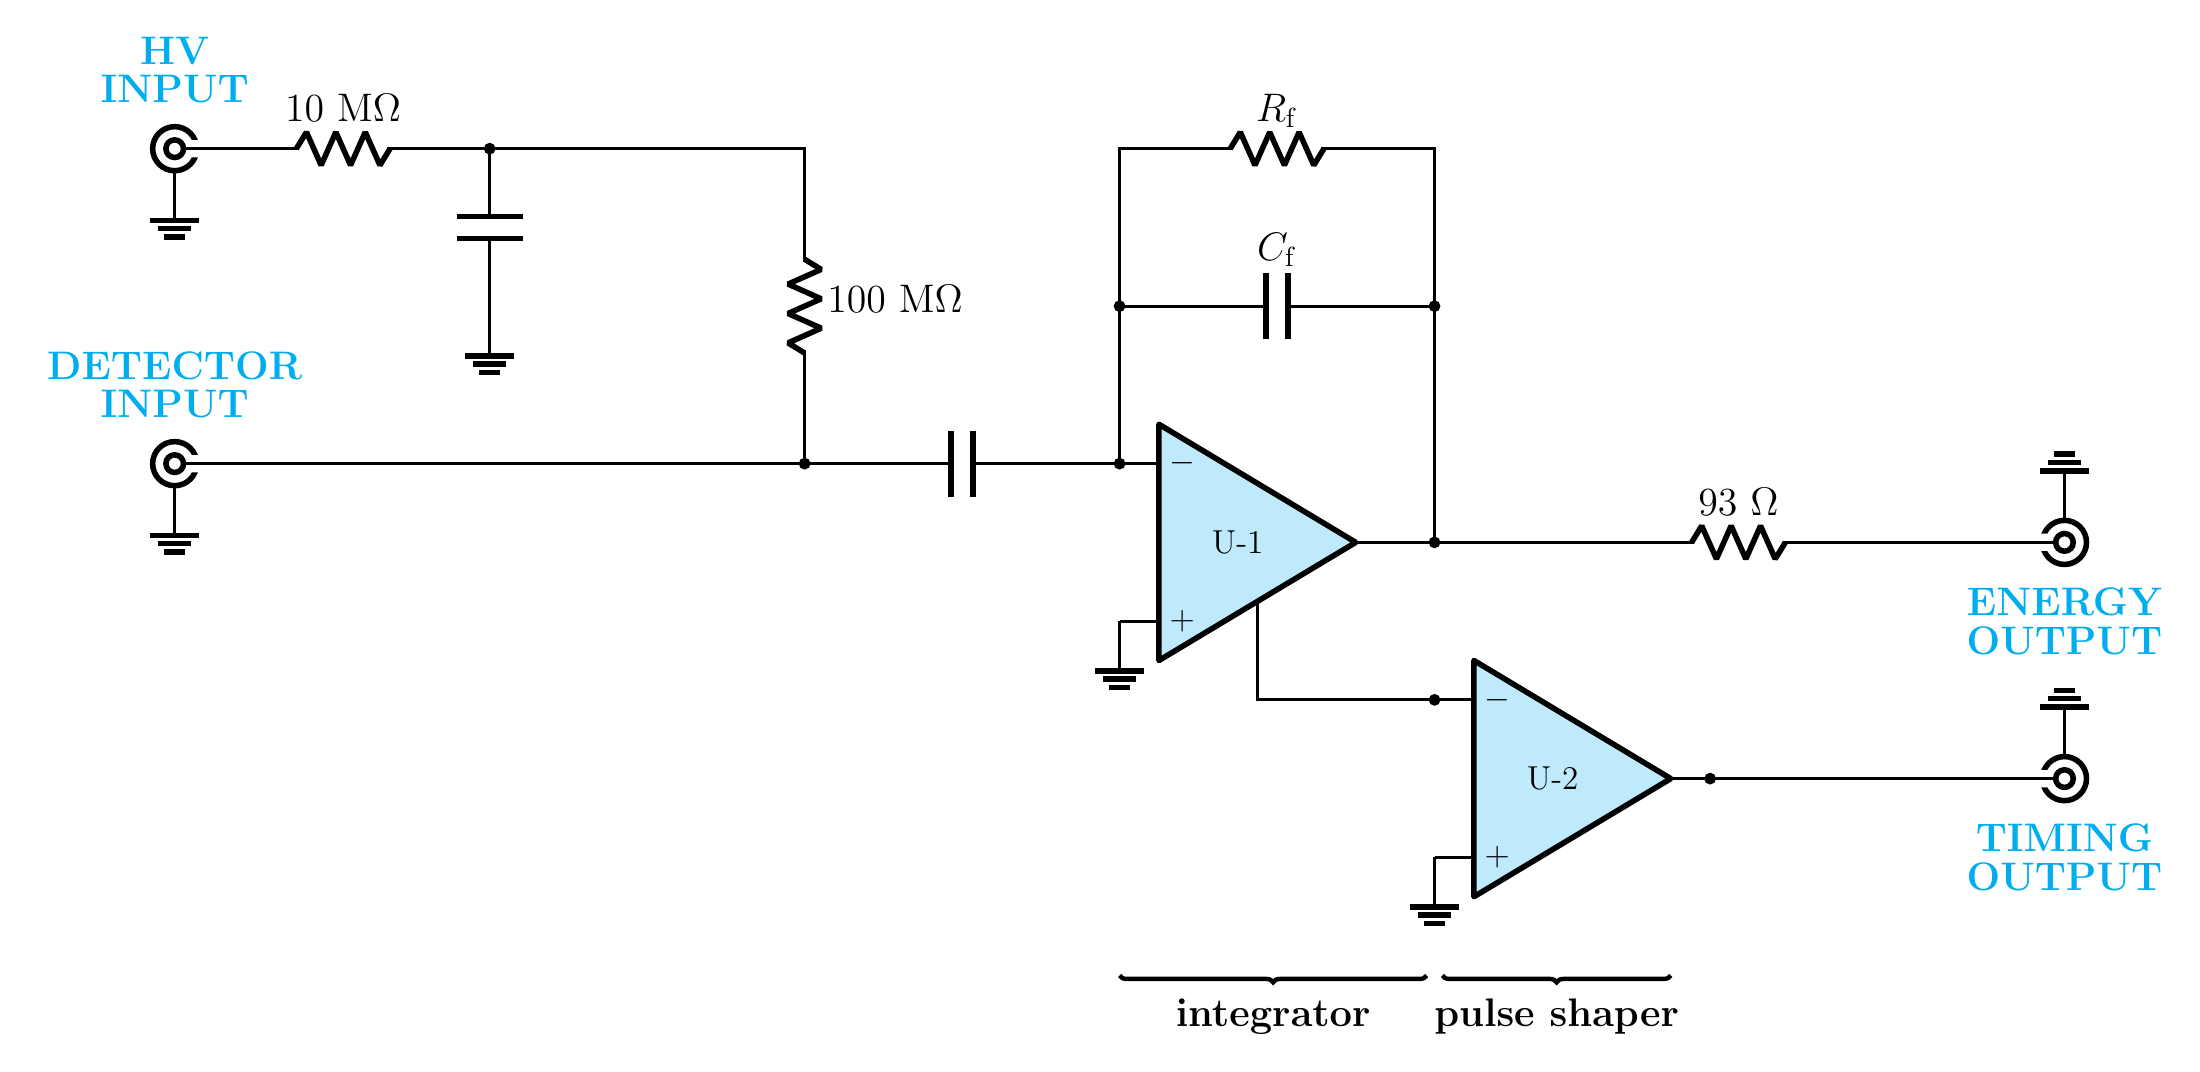
\begin{tikzpicture}[
        %Environment Config
        font=\large,
        MyArrow/.style={%Style for the current
            -Stealth,
            cyan,
            line width=1.0pt,
            shorten >= 5pt,
            shorten <= 1pt
        },
        Vref/.style={%Style for the voltage reference
            draw=none,
            postaction={decorate,decoration={markings,mark=at position 0.5 with {\node{\Large #1};}}},
            postaction={decorate,decoration={markings,mark=at position 0.15 with {\node{\Large $\bm{+}$};}}},
            postaction={decorate,decoration={markings,mark=at position 0.85 with {\node{\Large $\bm{-}$};}}}
        },
        Numbered/.style = {% Style for circle marks
                draw,
                circle,
                line width=1.5pt,
                align=center,
                inner sep=4pt,
                label distance=15pt
           }
    ]
    \def\MyOpamp(#1)#2{%Customized opamp
        \begin{scope}[shift={(#1)}]
            %Component Shape
            \draw[fill=cyan!25,line width = 2pt, line join=round] (0,0)++(-1,1.5)
                --++(2.5,-1.5) -- ++(-2.5,-1.5)-- cycle; 
            % Label and component identifier.
            \draw(0,0) node{U-#2}; % IC LABEL
            % Draw the pins
            % Some that you have to learn about label nodes, draw lines, and name coordinates in Tikz
            \draw[line width = 1pt] (-1,1) node [anchor=180]{$-$} -- ++(-0.5,0)  coordinate (#2 IN-); % IN - 
            \draw[line width = 1pt] (-1,-1) node [anchor=180]{$+$}  -- ++(-0.5,0) coordinate (#2 IN+); % IN +
            \draw[line width = 1pt] (1.5,0)  -- ++(0.5,0) coordinate (#2 OUT); % OUT  
        \end{scope}
    }
    \def\MyGround(#1)#2{%customized ground
        \begin{scope}[shift={(#1)}]
            %Component Shape
            \draw[line width = 2pt, line cap=round]
            (0,0) coordinate (#2 GND)++(-0.3,0)--++(0.6,0)
            (0,-0.15)++(-0.2,0)--++(0.4,0)
            (0,-0.3)++(-0.1,0)--++(0.2,0);  
        \end{scope}
    }
    
    
    %%%%%%%%%%%%%%%%%%%%%%%%%%%%%%%%%%%%%%%%%%%%%%%%%%%%%%%%%%%%%%%%%%%%%%%%%%%%
    % CIRCUIT
    %%%%%%%%%%%%%%%%%%%%%%%%%%%%%%%%%%%%%%%%%%%%%%%%%%%%%%%%%%%%%%%%%%%%%%%%%%%%
    % upper input part
    \draw[line width=1pt] (0,0) node[bnc, scale=2, anchor=zero] (UI1) {};
    \draw[line width=1pt] (0,1) node[scale=1.0, text width=2.5cm,align=center, anchor=center] (TUI1) {\color{cyan}\Large\bfseries HV\\INPUT};
    
    \draw[line width=1pt] (4,0) node[circ] (UI2) {};
    \draw[line width=1pt] (8,-4) node[circ] (UI3) {};
    \draw[line width=1pt] (0,-2) node (UITMP) {};
    % \draw node[ground, below=1cm] at (UI1.shield) (UGND1) {};
    % \draw node[ground] at (UI1.shield |- UITMP) (UGND1) {};
    \draw[line width=1pt] node[ground, scale=1.5] at (UI1.shield) (UGND1) {};
    % \draw node[ground] at (UI2 |- UITMP) (UGND2) {};
    \draw[line width=1pt] (4,-2) node[ground, scale=1.5] (UGND2) {};
    % \draw (UGND1) -- (UI1.shield);
    \draw[line width=1pt] (UGND2) to [C] (UI2); 
    \draw[line width=1pt] (UI1) to [R, l={\Large\( 10 \ \si{M\Omega} \)}] (UI2);
    \draw[line width=1pt] (UI2) -- (8,0) to [R, l={\Large\( 100 \ \si{M\Omega} \)}] (UI3);
    
    
    % lower input part
    \draw[line width=1pt] (0,-4) node[bnc, scale=2, anchor=zero] (LI1) {};
    \draw[line width=1pt] (0,-3) node[scale=1.0, text width=3.5cm,align=center, anchor=center] (TLI1) {\color{cyan}\Large\bfseries DETECTOR\\INPUT};

    \draw[line width=1pt] node[ground, scale=1.5] at (LI1.shield) (LGND1) {};
    \draw[line width=1pt] (LI1) -- (UI3);
    
    % middle input part
    \draw[line width=1pt] (12,-4) node[circ] (MI1) {};
    \draw[line width=1pt] (UI3) to [C] (MI1) {};
    \draw[line width=1pt] (12,-2) node[circ] (MI2) {};
    \draw[line width=1pt] (16,-2) node[circ] (MI3) {};
    \draw[line width=1pt] (16,-5) node[circ] (MI4) {};
    \draw[line width=1pt] (MI1) -- (MI2) -- (12,0) to [R, l={\Large\( R_{\mathrm{f}} \)}] (16,0) -- (MI3) -- (MI4);
    \draw[line width=1pt] (MI2) to [C, l={\Large\( C_{\mathrm{f}} \)}] (MI3);
    
    \MyOpamp(13.5,-5){1}
    \draw[line width=1pt] (15.5,-5) -- (MI4);
    \draw[line width=1pt] (16,-7) node[circ] (LO1) {};
    \draw[line width=1pt] node[ground, scale=1.5] at (12,-6) (MGND1) {};
    \draw[line width=1pt] (13.75,-5.75) -- (13.75,-7) -- (LO1);
    \draw[line width=1pt] (19.5,-8) node[circ] (LO2) {};
    \MyOpamp(17.5,-8){2}
    \draw[line width=1pt] node[ground, scale=1.5] at (16,-9) (OGND1) {};
    
    \draw[line width=1pt] (24,-5) node[bnc, scale=2, anchor=zero, rotate=-180] (UO1) {};
    \draw[line width=1pt] (24,-6) node[scale=1.0, text width=2.5cm, align=center, anchor=center] (TUO1) {\color{cyan}\Large\bfseries ENERGY\\OUTPUT};
    
    \draw[line width=1pt] (24,-8) node[bnc, scale=2, anchor=zero, rotate=-180] (LO3) {};
    \draw[line width=1pt] (24,-9) node[scale=1.0, text width=2.5cm, align=center, anchor=center] (TLO3) {\color{cyan}\Large\bfseries TIMING\\OUTPUT};

    \draw[line width=1pt] node[ground, scale=1.5, rotate=-180] at (UO1.shield) (OGND2) {};
    \draw[line width=1pt] node[ground, scale=1.5, rotate=-180] at (LO3.shield) (OGND3) {};
    \draw[line width=1pt] (LO2) -- (LO3);
    \draw[line width=1pt] (MI4) to [R, l={\Large\( 93 \ \si{\Omega} \)}] (UO1);
    
    % underbraces
    \draw[
        ultra thick,
        decoration={
            brace,
            mirror,
            raise=0.5cm
        },
        decorate
    ] (12,-10) -- (15.9,-10) node [pos=0.5, anchor=north, yshift=-0.65cm] {\Large\bfseries integrator};
    \draw[
        ultra thick,
        decoration={
            brace,
            mirror,
            raise=0.5cm
        },
        decorate
    ] (16.1,-10) -- (19,-10) node [pos=0.5, anchor=north, yshift=-0.65cm] {\Large\bfseries pulse shaper};
    \end{tikzpicture}
    % \begin{tikzpicture}[
    %     %Environment Config
    %     font=\large,
    %     MyArrow/.style={%Style for the current
    %         -Stealth,
    %         cyan,
    %         line width=1.5pt,
    %         shorten >= 5pt,
    %         shorten <= 1pt
    %     },
    %     Vref/.style={%Style for the voltage reference
    %         draw=none,
    %         postaction={decorate,decoration={markings,mark=at position 0.5 with {\node{\Large #1};}}},
    %         postaction={decorate,decoration={markings,mark=at position 0.15 with {\node{\Large $\bm{+}$};}}},
    %         postaction={decorate,decoration={markings,mark=at position 0.85 with {\node{\Large $\bm{-}$};}}}
    %     },
    %     Numbered/.style = {% Style for circle marks
    %             draw,
    %             circle,
    %             line width=1.5pt,
    %             align=center,
    %             inner sep=4pt,
    %             label distance=15pt
    %       }
    % ]
    % \def\MyOpamp(#1)#2{%Customized opamp
    % \begin{scope}[shift={(#1)}]
    % %Component Shape
    % \draw[fill=cyan!25,line width = 2pt, line join=round] (0,0)++(-1,1.5)
    %     --++(2.5,-1.5) -- ++(-2.5,-1.5)-- cycle; 
    % % Label and component identifier.
    % \draw(0,0) node{\sf U-#2}; % IC LABEL
    % % Draw the pins
    % % Some that you have to learn about label nodes, draw lines, and name coordinates in Tikz
    % \draw[line width = 1.5pt] (-1,1) node [anchor=180]{$-$} -- ++(-0.5,0)  coordinate (#2 IN-); % IN - 
    % \draw[line width = 1.5pt] (-1,-1) node [anchor=180]{$+$}  -- ++(-0.5,0) coordinate (#2 IN+); % IN +
    % \draw[line width = 1.5pt] (1.5,0)  -- ++(0.5,0) coordinate (#2 OUT); % OUT  
    % \end{scope}
    % }
    % \def\MyGround(#1)#2{%customized ground
    % \begin{scope}[shift={(#1)}]
    % %Component Shape
    % \draw[line width = 2pt, line cap=round]
    % (0,0) coordinate (#2 GND)++(-0.3,0)--++(0.6,0)
    % (0,-0.15)++(-0.2,0)--++(0.4,0)
    % (0,-0.3)++(-0.1,0)--++(0.2,0);  
    % \end{scope}
    % }

    % %Put the customzed opamp in position
    % \MyOpamp(0,0){1}

    % %Put some short nodes
    % \draw(-7,1) node[ocirc,scale=2,line width=1.5pt](N3){};
    % \draw(-3,1) node[circ,scale=2,line width=1.5pt](N2){};
    % \draw(3,0) node[circ,scale=2,line width=1.5pt](N6){};
    % \draw(5.5,0) node[ocirc,scale=2,line width=1.5pt](N6-OUT){};
    % \MyGround(-7,-3){1}
    % \MyGround(1 GND -| N2){2}
    % \MyGround(1 GND -| N6-OUT){3}

    % %Draw the Wires and pasive components
    % \draw[line width=1.5pt]
    % (N3)%From node N3
    %     --++(1,0)
    %     to [R,l=\Large$R_1$] (N2)
    %     --(1 IN-)
    % (N2)
    %     --++(0,2) coordinate (N5)
    %     --++(2.5,0)
    %     to[R,l=\Large$R_2$]++(3,0)
    %     -| (N6)
    % (1 OUT) 
    %     -- (N6-OUT)
    % (1 IN+)
    %     -|(2 GND);
    % %Voltage references
    % \draw[Vref=$v_1$]
    % (N3) 
    %     -- (1 GND);

    % \draw[Vref=$0$ V,color=cyan]
    % (1 IN-)
    %     ++(-0.5,0) coordinate (temp) 
    %     -- (1 IN+ -| temp)
    %     node[
    %         midway,
    %         label={[Numbered,black]180:\bf 1}
    %     ]{};

    % \draw[Vref,color=cyan]
    % (N6-OUT) 
    %     -- (3 GND) 
    %     node [
    %         midway,
    %         anchor=west,
    %         label={[Numbered,black,label distance=5pt]180:\bf 6}
    %     ]{$\bm{v_o} = 0-\cfrac{v_1}{R_1}R_2$};

    % \draw[MyArrow]
    % (N2)++(-1.5,-5) 
    %     node [
    %         label={[Numbered,black,label distance=5pt]180:\bf 2}
    %     ](C1){$\bm{v_1} = 0$ \bf (Virtual ground)}
    % (C1.168) %get a point from center to node box at 168 degrees
    %     to [out=80, in=-150] (N2);

    % %Draw currents
    % \draw[MyArrow]
    % (N3)++(0.3,0.3)
    %     -- ++(1.5,0)
    %     node [
    %         midway,
    %         inner sep=10pt,
    %         anchor=-70,
    %         label={[Numbered,black,label distance=0pt]180:\bf 3}
    %     ]{$\bm{i_1} = \cfrac{v_1}{R_1}$};

    % \draw[MyArrow]
    % (N2)++(0.5,0.3)
    %     -- ++(1.2,0)
    %     node [
    %         midway,
    %         inner sep=10pt,
    %         anchor=-70,
    %         label={[Numbered,black,label distance=0pt]12:\bf 4}
    %     ]{$0$};
    % \draw[MyArrow]
    % (N5)++(0.3,0.3) %node gap
    %     -- ++(2,0) % Arrow longitude
    %     node [
    %         midway,
    %         inner sep=10pt,
    %         anchor=-70,
    %         label={[Numbered,black,label distance=0pt]180:\bf 5}
    %     ]{$\bm{i_2} = \bm{i_1} =\cfrac{\bm{v_1}}{R_1}$};
    % \draw[cyan]
    % (C1 -| 3 GND)
    %     node [
    %         inner sep=10pt,
    %         anchor=west,
    %     ]{$\bm{v_o} = -\cfrac{R_2}{R_1}v_i$};

    % \end{tikzpicture}
\end{document}